\documentclass{article}
\usepackage{preamble}
\usepackage{env}
\usepackage{configure}

% available environments:
% theorem: thm
% definition: defn
% proof: pf
% corollary: crll
% lemma: lm
% question: qu
% solution: soln
% example: xmp
% exercise: exr
%
% options: title=<title>   {all}
%          source=<source> {pf, qu, soln, xmp, exr}  Note: if content is taken directly from the main resource, cite the main resource as ``Primary source material"


% define these variables!
\def\coursecode{MAT257Y5}
\def\coursename{} % use \relax for non-course stuff
\def\studytype{} % 1: Personal Self-Study Notes / 2: Course Lecture Notes / 3: Revised Notes / 4: Exercise Solution Sheet
\def\author{\me}
\def\createdate{}
\def\updatedate{\today}
\def\source{} % name, ed. of textbook, or `Class Lectures` for class notes
\def\sourceauthor{} % for class notes, put lecturer
\def\leftmark{Week 9 - Total Differentiability} % set text in header; should only be necessary in assignments etc.
\pagenumbering{arabic} % force revert numbering to default; should only be necessary in assignments etc.

\begin{document}

\setcounter{subsection}{7}
\setcounter{qu}{6}

\begin{qu}
    Recall the function $ \alpha: \bb{R} \rightarrow \bb{R} $ as given in Big List 4(a):
    \begin{equation*}
    \alpha(x) = \begin{cases} 0 & x \leq 0 \\ e^{-1/x} & x > 0 \end{cases}
    \end{equation*}
    %
    Let $ f: \bb{R}^{2} \rightarrow \bb{R} $ be the function given by:
    \begin{equation*}
        f(\vec p) = \frac{2\alpha\left(\frac{1+\norm{\vec p}}{2}\right)}
        {\alpha\left( \frac{1+\norm{\vec p}}{2}\right)
        + \alpha\left( \frac{1 - \norm{\vec p}}{2} \right)} - 1
    \end{equation*}
    Show that $ f $ is continuous, but not totally differentiable, at $ (0, 0) $.
\end{qu}

\begin{soln}
    Here's a picture of the function: \vsp

    \centering
    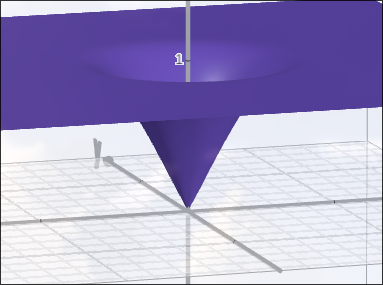
\includegraphics[width=0.3\linewidth]{figures/sinkhole.png}
    \flushleft

    We see that when $ \vec p \neq \vec{0} $, then $ f $ is the composition of several
    continuous functions and is therefore continuous. At $ \vec{p} = \vec{0} $, we get that:
    \begin{align*}
        f(\vec{0}) & = \frac{2\alpha\left(\frac{1}{2}\right)}
        {\alpha\left( \frac{1}{2}\right)
        + \alpha\left( \frac{1}{2} \right)} - 1 \vsp
                   & = \frac{2\alpha \left( \frac{1}{2} \right)}
                   {2\alpha \left( \frac{1}{2} \right)} - 1 \vsp
                   & = 0
    \end{align*}
    So again by continuity of the composed functions, $ f $ is also continuous at $ 0 $. \vsp
    %
    (We'll drop the vector arrows from here on out.)
    To see that it is not totally differentiable at $ 0 $, suppose by contradiction it is.
    Then, there exists some $ L : \bb{R}^{2} \rightarrow \bb{R} $ such that:
    \begin{equation*}
        \lim_{h \rightarrow 0} \frac{\abs{f(0 + h) - f(0) - L(h)}} {\norm{h}}
        = \lim_{h \rightarrow 0} \frac{\abs{f(h) - L(h)}}{\norm{h}} = 0
    \end{equation*}
    By the reverse triangle inequality, we have that:
    \begin{equation*}
        \frac{1}{\norm{h}}\abs{f(h) - L(h)} \geq \frac{1}{\norm{h}}\abs{\abs{f(h)} - \abs{L(h)}}
        \geq \frac{1}{\norm{h}}\abs{\abs{f(h)} + M\norm{h}} = \abs{\frac{\abs{f(h)}}{\norm{h}} + M}
        \geq \frac{\abs{f(h)}}{\norm{h}}
    \end{equation*}
    So it suffices to show that as $ h \rightarrow 0, \dfrac{\abs{f(h)}}{\norm{h}}
    \cnot\rightarrow 0 $.
    \newpage

    Denote $ x = \norm{h} $ and $ y = \dfrac{2x}{1-x^{2}} $.
    Then, with some very extensive algebra, we have on $ [0, 1) $ that:
    \begin{align*}
        \frac{\abs{f(h)}}{x} & = \frac{1}{x} \cdot
        \frac{2e^{\frac{-2}{1+x}}}{e^{\frac{-2}{1+x}} + e^{\frac{-2}{1-x}}} - 1 \vsp
                             & = \frac{1}{x} \cdot
        \frac{e^{\frac{2}{1-x}} - e^{\frac{2}{1+x}}}{e^{\frac{2}{1-x}} + e^{\frac{2}{1+x}}} \vsp
                             & = \frac{1}{x} \cdot
        \frac{e^{\frac{2(1+x)}{1-x^{2}}} - e^{\frac{2(1-x)}{1-x^{2}}}}
        {e^{\frac{2(1+x)}{1-x^{2}}} + e^{\frac{2(1-x)}{1-x^{2}}}} \vsp
                             & = \frac{1}{x} \cdot
        \frac{e^{\frac{2+2x}{1-x^{2}}} - e^{\frac{2-2x}{1-x^{2}}}}
        {e^{\frac{2+2x}{1-x^{2}}} + e^{\frac{2-2x}{1-x^{2}}}} \vsp
                             & = \frac{1}{x} \cdot
        \frac{e^{\frac{2}{1-x^{2}}}\left( e^{\frac{2x}{1-x^{2}}} - e^{\frac{-2x}{1-x^{2}}} \right)}
        {e^{\frac{2}{1-x^{2}}}\left( e^{\frac{2x}{1-x^{2}}} + e^{\frac{-2x}{1-x^{2}}} \right)} \vsp
                             & = \frac{1}{x} \cdot
        \frac{e^{y} - e^{-y}}{e^{y} + e^{-y}} \vsp
                             & = \frac{1}{x} \tanh(y) \vsp
                             & = \frac{1}{x} \tanh \left( \frac{2x}{1-x^{2}} \right)
    \end{align*}
    We use L'Hopital's to see that the limit is given by:
    \begin{equation*}
        \lim_{x \rightarrow 0^{+}} \frac{1}{x}\tanh \left( \frac{2x}{1-x^{2}} \right)
        \ = \ \lim_{x \rightarrow 0^{+}} \sech^{2}\left( \frac{2x}{1-x^{2}} \right) \cdot
        \frac{2(1-x^{2}) + 4x}{(1-x^{2})^{2}}
    \end{equation*}
    The above is continuous on $ [0, 1) $, and expands to:
    \begin{equation*}
        \sech^{2}(y) \cdot \frac{2(1-x^{2}) + 4x}{(1-x^{2})^{2}}
        \ = \ \frac{4e^{2y}}{(e^{2y} +1)^{2}} \cdot \frac{2(1-x^{2}) + 4x}{(1-x^{2})^{2}}
    \end{equation*}
    At $ x = 0 $, we have that $ y = 0 $ as well. Putting it all together, we have that:
    \begin{equation*}
        \lim_{h\rightarrow0} \frac{\abs{f(h) - L(h)}}{\norm{h}}
        \ \geq \ \lim_{h\rightarrow0} \frac{\abs{f(h)}}{\norm{h}}
        \ = \ \frac{4 \cdot 1}{(1 + 1)^{2}} \cdot \frac{2(1) + 4 \cdot 0}{(1 - 0)^{2}}
        \ = \ 1 \cdot 2 \ = \ 2 \ \neq \ 0
    \end{equation*}
    We finally arrive at our contradiction, showing that $ f $ is not totally differentiable
    at the origin.
\end{soln} \vspace{-2mm}
\begin{lm}[type=Conjecture.]
    Let $ U \subseteq \bb{R}^{n} $ be an open neighbourhood containing the origin.
    Given two continuous functions $ f, g : U \rightarrow \bb{R}^{m} $, suppose there exists
    a real number $ c > 0 $ satisfying the condition that: \vspace{-1mm}
    \begin{equation*}
        \lim_{x \rightarrow 0}\frac{\norm{f(x)}}{\norm{g(x)}} = c
    \end{equation*}
    Then $ f $ is differentiable at $ 0 $ if and only if $ g $ is differentiable at $ 0 $.
\end{lm}

\end{document}
